\documentclass[a4paper,11pt]{article}
\usepackage[utf8]{inputenc}
\usepackage[italian]{babel}
\usepackage[margin=1.5cm,top=1.5cm,bottom=1.5cm]{geometry}
\usepackage{tikz,graphicx,amsmath,amssymb,booktabs,xcolor}
\usepackage{helvet}
\renewcommand{\familydefault}{\sfdefault}
\pagestyle{empty}
\begin{document}

\begin{minipage}[t][0.18\textheight]{\textwidth}
  \centering
  {\huge\bfseries (34713) Yesiltas occults GAIA 3367029716095038976}\\[0.4cm]
  {\large 2026-05-25 20:22:57 UT}\\[0.4cm]
  \begin{tabular}{p{0.3\textwidth} p{0.3\textwidth} p{0.3\textwidth}}
    \textbf{Asteroide} & \textbf{Stella} & \textbf{Evento} \\
    \midrule
    Diametro: 5.8 km & Mag: 17.4 & Calo mag: 2.3 \\
    Mag (H): 13.86 & RA: +108°06'58.05" & Durata max: 0.2 s \\
    Albedo: 0.398 & Dec: +21°10'44.35" & Incertezza: $\pm$83082 km \\
  \end{tabular}
\end{minipage}
\vfill

\begin{minipage}[t][0.38\textheight]{\textwidth}
  \begin{minipage}[t]{0.48\textwidth}
    \centering
    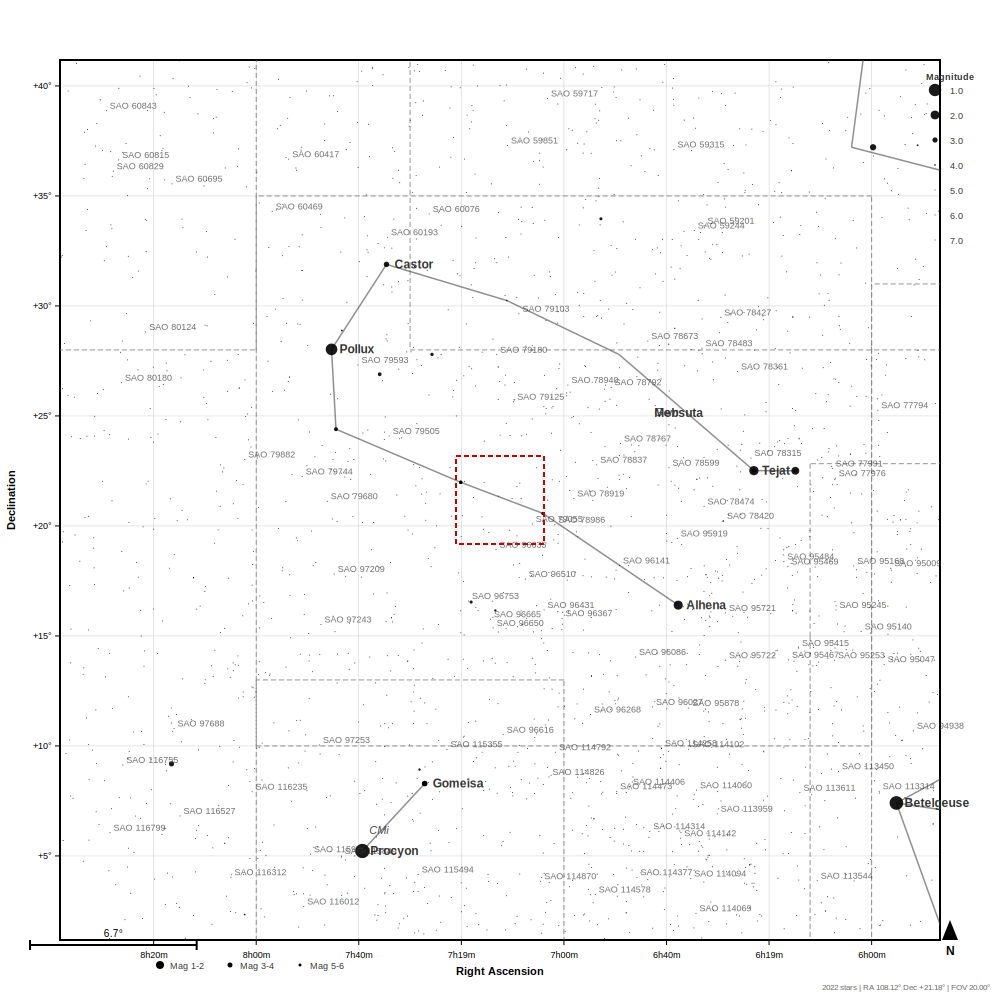
\includegraphics[width=\textwidth]{card_A4_34713_GAIA_DR3_3367029716095038976_approach.png}
  \end{minipage}
  \hfill
  \begin{minipage}[t]{0.48\textwidth}
    \centering
    \includegraphics[width=\textwidth]{card_A4_34713_GAIA_DR3_3367029716095038976_earth.png}
  \end{minipage}
\end{minipage}
\vfill

\begin{minipage}[t][0.38\textheight]{\textwidth}
    \centering
    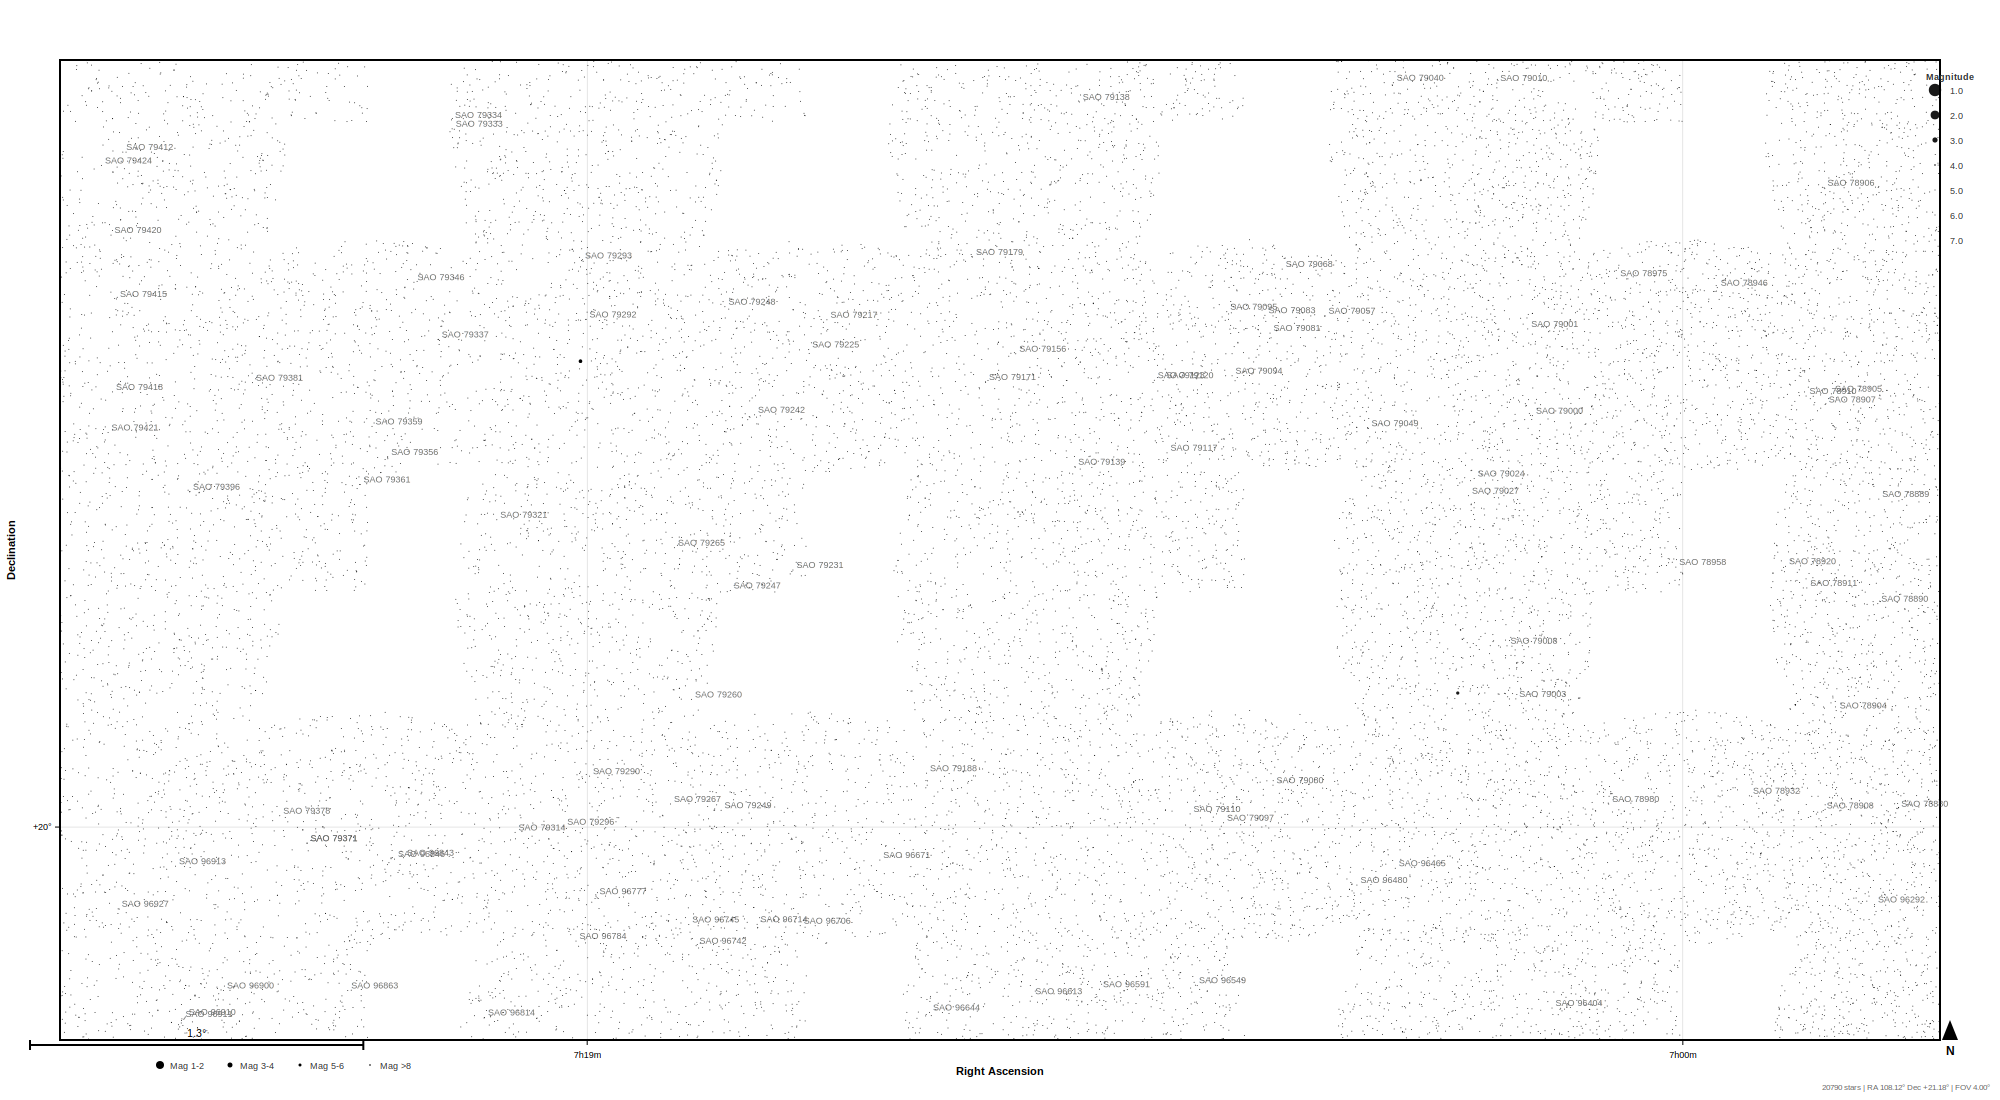
\includegraphics[width=\textwidth,height=0.34\textheight,keepaspectratio]{card_A4_34713_GAIA_DR3_3367029716095038976_finder.png}
\end{minipage}
\end{document}
